\section{Experiment}
\paragraph{}
This experiment followed strict patterns to ensure that it would not affect the servers of each of the tested solutions. No real data was used in the tests. Each solution got an account created and the same set of dummy data inserted into it.


\subsection{Testing environment}
\paragraph{}
The research will be conducted within a client-server environment. In this research we will be using five servers with the following specifications:
\begin{itemize}
	\item Intel Xeon processor
	\item 8GB ram
	\item SSD + HDD for storage
\end{itemize}

\subsubsection{Physical server}
 We used four physical servers to setup the needed services. Additional tools will be used, as well multiple logging and bench marking tools that allow us to keep a detailed log on the resource consumption and performance measurement. The fifth physical server is used for building the virtual setup.

\subsubsection{Virtual server}
\paragraph{}
For the virtual server we will be using Xen 4.8.2 as hypervisor to implements the VMs. On top of the hypervisor there is a Dom0.
 
\subsubsection{Setup overview}
\begin{figure}[H]
    \centering
    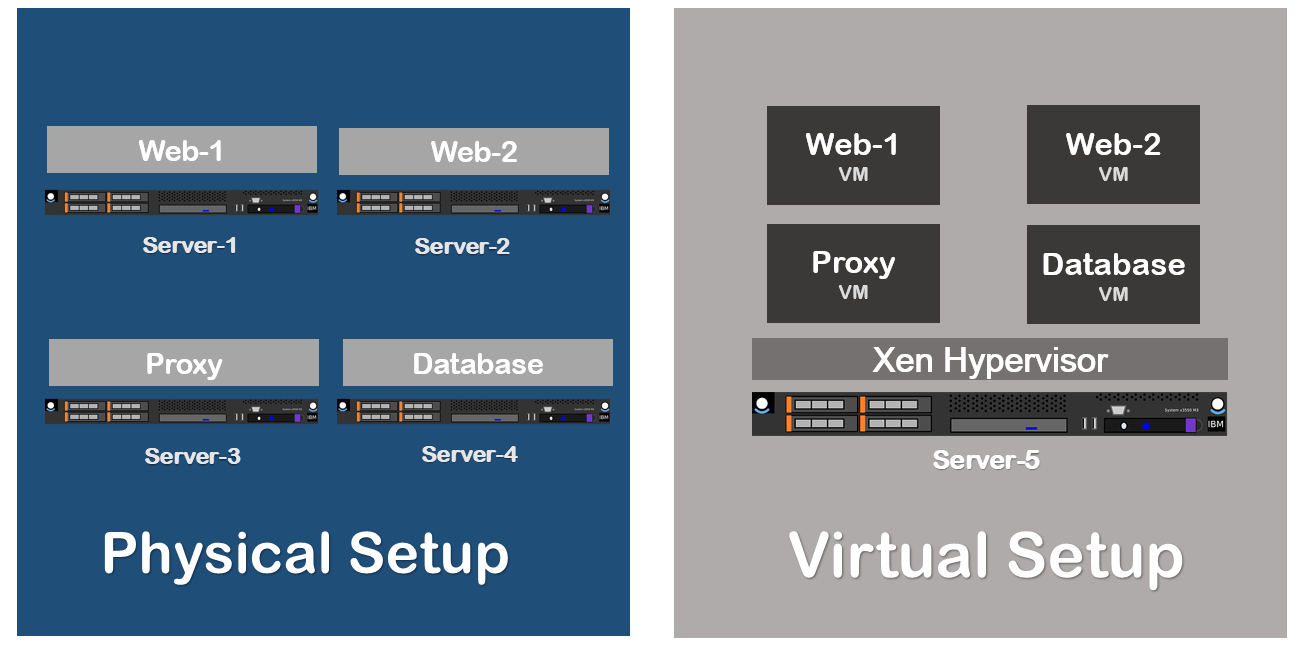
\includegraphics[width=14cm]{Pictures/setup.PNG}
    \caption{Test Environment Setup}
    \label{fig:setupoverview}
\end{figure}

The \textbf{figure \ref{fig:setupoverview}} above illustrates both the physical and virtual setups environment, in addition to each service that run on which server. The networking between the servers on the physical setup is also physical. The networking between the virutal servers is virtualized by using a Xenbridge.

\subsection{Web application}
For the application part of our setup, we used osCommerce\cite{oscommerce}, as shown in \textbf{figure \ref{fig:osCommerce}}. OsCommerce is an opensouce webstore conternt management used in many webshops. It runs on a webserver and uses PHP and MySQL. As webserver we used Apache (Apache/2.4.18) with the PHP (7.0.22-0)  extention. For the database we used MySQL(5.7.20-0). The proxyserver runs nginx(1.10.3). The setup for the Hardware and VM are the same. It provides a realistic web application.

\begin{figure}[H]
    \centering
    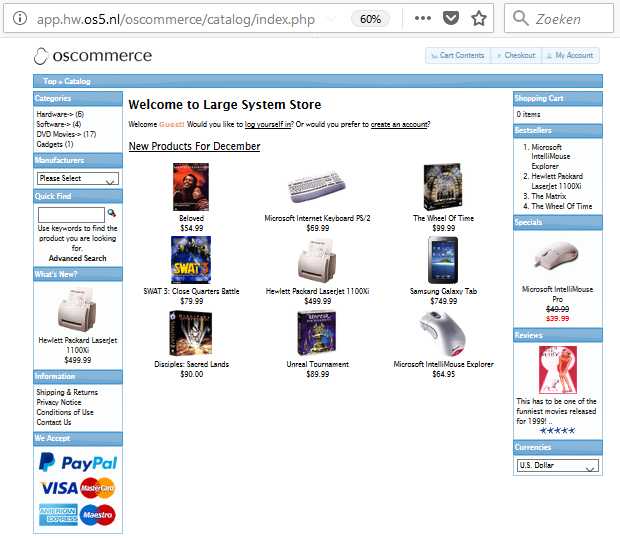
\includegraphics[width=10cm]{Pictures/oscom.PNG}
    \caption{Large System Store \- Powered by osCommerce}
    \label{fig:osCommerce}
\end{figure}

\subsection{Tools}
\paragraph{}
In order to achieve a consistent and precise output for our experiments. We used two different tools run on different operating systems to load and stress our setup. The tools are the following: 

\begin{itemize}
\item The former one is \textbf{Apache HTTP server benchmarking tool} which is an open source Linux based tool. It is "a tool for benchmarking your Apache Hypertext Transfer Protocol (HTTP) server. It is designed to give you an impression of how your current Apache installation performs. This especially shows you how many requests per second your Apache installation is capable of serving" \cite{ab}. 

\item The latter one is \textbf{Paessler Webserver Stress Tool} which is Windows based free performance, load, and stress-test for web servers. It is a powerful HTTP-client/server test application designed to pinpoint critical performance issues in your web site or web server that may prevent optimal experience for your site's visitors. It  simulates "the HTTP requests generated by hundreds or even thousands of simultaneous users, you can test your web server performance under normal and excessive loads to ensure that critical information and services are available at speeds your end-users expect" \cite{paessler}.
\end{itemize}

\subsection{Methodology}
\paragraph{}
In this project we followed a methodology that starts from basic tests to increasingly complex ones on both virtual and physical servers. The steps we followed were:
\begin{itemize}
    \item \textbf{Basic setup tests:}
 In the basic setup tests we used only the Apache HTTP server benchmarking tool to experiment the web server alone by itself without the complete setup as illustrated in the \textbf{figure \ref{fig:setupbasic}}. 
 We targeted only the static web page of our osCommerce store.
 \begin{figure}[H]
    \centering
    
\includegraphics[width=6cm]{Pictures/simple.PNG}
    \caption{Basic Setup Test Methodology}
    \label{fig:setupbasic}
\end{figure}

\item \textbf{Full setup tests:}
 For the complete setup test we used both the Apache HTTP server benchmarking tool and Paessler webserver Stress tool to experiment the complete setup environment which includes proxy, web, and database servers as shown in \textbf{figure \ref{fig:setupfull}}. 
 We targeted the proxy server which acts as load balancer between our two webservers. And these two webservers interact directly with the database server. Which leads to a complete setup tests.   
 
 \begin{figure}[H]
    \centering
    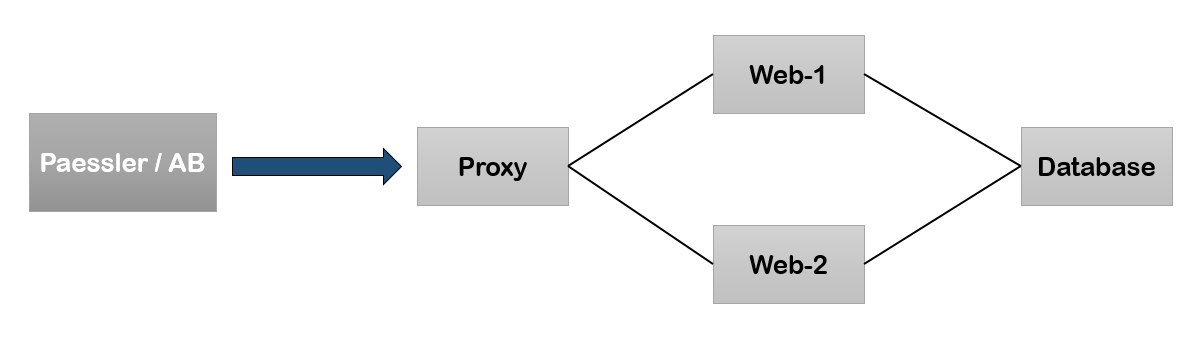
\includegraphics[width=12cm]{Pictures/complex.PNG}
    \caption{Full Setup Test Methodology}
    \label{fig:setupfull}
\end{figure}
\end{itemize}

\subsection{Naming structure}
\paragraph{}
For the project we used the following url structure, to prevent mistakes during the measurement. Fully Qualified Domain Name (FQDN) of the servers used:
$$\begin{Bmatrix}app \mid web1 \mid web2 \mid db \end{Bmatrix} .  \begin{Bmatrix} vm \mid hw \end{Bmatrix} . os5 . nl .$$
\paragraph{}
For the static web page:\\
$$ \begin{bmatrix}
 http://  \begin{Bmatrix}app \mid web1 \mid web2 \end{Bmatrix} .  \begin{Bmatrix} vm \mid hw \end{Bmatrix} . os5 . nl 
  \\ \vdots \\ http://web1.hw.os5.nl
\end{bmatrix}$$
\paragraph{}
For the dynamic web page:\\
$$ \begin{bmatrix}
http://  \begin{Bmatrix}app \mid web1 \mid web2 \end{Bmatrix} .  \begin{Bmatrix} vm \mid hw \end{Bmatrix} . os5 . nl /  oscommerce / catalog / \begin{Bmatrix} php script \end{Bmatrix}   \\ \vdots \\
http://  app .  vm . os5 . nl /  oscommerce / catalog / product\_info.php?products\_id=25   
\end{bmatrix}$$